\documentclass[10pt,a4paper]{article}
\usepackage[utf8]{inputenc}
\usepackage[french]{babel}
\usepackage[T1]{fontenc}
\usepackage{amsmath}
\usepackage{amsfonts}
\usepackage{amssymb}
\usepackage{graphicx}
\usepackage[left=2cm,right=2cm,top=2cm,bottom=2cm]{geometry}
\usepackage{physics} %Physics.sty
\author{Loann Brahimi}
\title{Calcul du taux d'amortissement des ondes de Alfvén par collisions ions-neutres}
\begin{document}
\maketitle 

\section*{Coefficients d'amortissement par collisions ions-neutres}

Dans ce document nous allons calculer le coefficient d'amortissement des ondes de Alfvén par collisions des ions avec les neutres dans le cadre d'un milieu faiblement ionisé. On écrit dans un premier temps la relation de dispersion des ondes de Alfvén incluant un amortissement suivant les collisions neutre-ion et la viscosité des neutres. On a (Xu 2015) :

\begin{equation}
	\omega^3 + i\left({\tau_v}^{-1} + (1+\chi)\nu_{ni}\right)\omega^2 - \left(k^2\cos^2{\theta} {V_{Ai}}^2 + 
	\chi{\tau_v}^{-1}\nu_{ni}\right)\omega - i\left({\tau_v}^{-1} + \nu_{ni}\right)k^2\cos^2{\theta} {V_{Ai}}^2 = 0
	\label{1}
\end{equation}

où $\chi = \rho_n / \rho_i$ et ${\tau_v}^{-1} = k^2 \nu^n$. Dans un premier temps, on néglige la viscosité cinématique des neutres $\nu_n \approx 0$, l'équation \ref{1} devient : 

\begin{equation}
	\omega^3 + i(1+\chi)\nu_{ni}\omega^2 - k^2\cos^2{\theta} {V_{Ai}}^2\omega - i\nu_{ni}k^2\cos^2{\theta} {V_{Ai}}^2 = 0
	\label{2}
\end{equation}

Xu+2015 propose des solutions analytiques dans le cas d'un amortissement faible c'est à dire $\abs{\Gamma_{in}} \ll \abs{\omega_R}$. 

\begin{eqnarray}
	{\omega_R}^2 & = & \frac{k^2\cos^2{\theta}{V_{Ai}}^2 \left[(1+\chi){\nu_{ni}}^2 + k^2 \cos^2{\theta} {V_{Ai}}^2\right]}{(1+\chi)^2{\nu_{ni}}^2 + k^2 \cos^2{\theta} {V_{Ai}}^2} \\
	\Gamma_{in}  & = & - \frac{\nu_{ni}\chi  k^2 \cos^2{\theta} {V_{Ai}}^2}{2\left[ (1+\chi)^2{\nu_{ni}}^2 + k^2 \cos^2{\theta} {V_{Ai}}^2 \right]}
\end{eqnarray}

Dans le cas d'un couplage fort ($\omega \ll \nu_{in}$) on a : 

\begin{eqnarray}
	{\omega_R}^2 & = & {V_{A}}^2 k^2 \cos^2{\theta} \\ 
	\Gamma_{in}  & = & - \frac{\xi_n  {V_{A}}^2 k^2 \cos^2{\theta}}{2 \nu_{ni}}
\end{eqnarray}

\begin{figure}[h]
\center
\begin{tabular}{|c|c|}
\hline 
\multicolumn{2}{|c|}{$\Gamma_{in} = - \frac{\xi_n V^2_A k^2 \cos^2{\theta} }{2 \nu_{ni}}$ Modes slab $\cos{\theta} = 1$ } \\ 
\hline 
WNM & $\Gamma^{\mathrm{WNM}}_{in} = - \left[ 3.0 \times 10^5 \left( \frac{k}{10^{-9}~\mathrm{cm}^{-1}} \right)^2 - 3.67 \times 10^6 \left( \frac{k}{10^{-9}~\mathrm{cm}^{-1}} \right)^2 \right]~ \mathrm{s}^{-1}$ \\ 

CNM & $\Gamma^{\mathrm{CNM}}_{in} = - \left[ 4.35 \times 10^4 \left( \frac{k}{10^{-9}~\mathrm{cm}^{-1}} \right)^2 - 1.72 \times 10^6 \left( \frac{k}{10^{-9}~\mathrm{cm}^{-1}} \right)^2 \right]~ \mathrm{s}^{-1}$ \\ 

MM & $\Gamma^{\mathrm{MM}}_{in} \approx  - 4.5 \times 10^7 \left( \frac{k}{10^{-9}~\mathrm{cm}^{-1}} \right)^2~ \mathrm{s}^{-1} $ \\ 
\hline 
\end{tabular} 

\caption{Tableau récapitulant les différents taux d'amortissement des ondes de Alfvén dans le cas d'un couplage faible. Ces derniers sont paramétrisés suivant l'échelle $k$. Les données proviennent de Jean + 2009, sauf pour le terme $\expval{\sigma v}$ qui est issu de Kulsrud + 1971. Enfin, la densité volumique de neutres dans le cas des nuages moléculaires à été prise de la thèse de Koertgen.}
\end{figure}

Dans le cas d'un couplage faible ($\omega \gg \nu_{in}$) on a : 

\begin{eqnarray}
	{\omega_R}^2 & = & {V_{Ai}}^2 k^2 \cos^2{\theta} \\ 
	\Gamma_{in}  & = & - \frac{\nu_{in}}{2} \label{taux_fort}
\end{eqnarray}

avec $\nu_{in} = \frac{m_n}{m_i + m_n}n_n \expval{\sigma v}$.  \\ 

\begin{figure}
\center
\begin{tabular}{|c|c|}
\hline 
\multicolumn{2}{|c|}{$\Gamma_{in} = - \frac{\nu_{in}}{2}$} \\ 
\hline 
WNM & ${\Gamma_{in}}^{\mathrm{WNM}} \sim - \left( 10^{-9} - 3.5 \times 10^{-9} \right)~\mathrm{s}^{-1}$ \\  
CNM & ${\Gamma_{in}}^{\mathrm{CNM}} \sim - \left( 1.5\times 10^{-8} - 4.0 \times 10^{-8} \right)~\mathrm{s}^{-1}$ \\ 
MM & ${\Gamma_{in}}^{\mathrm{MM}} \sim - \left( 0.5 \times 10^{-7} - 0.5 \times 10^{-3} \right)~\mathrm{s}^{-1}$ \\ 
\hline 
\end{tabular}
\caption{Taux d'amortissement des ondes de Alfvén dans les phases WNM, CNM, MM de l'ISM. Les données utilisées pour effectuer le calcul des taux sont issues de Jean et al. (2009) table 1. et paragraphe 2.1. Ce taux est obtenu dans le cas d'un couplage ions-neutre fort ($\omega \gg \nu_{in}$). } 
\end{figure}

\section*{Détermination du taux de turbulence}

On peut également, en suivant la méthode utilisée par Wiener + 2013, déterminer le taux de turbulence $b_k = \delta B / B_0$ à partir de la condition d'équilibre des ondes de Alfvén entre taux de croissance et taux d'amortissement par collision ions-neutres. Les formules (26) et (25) de Wiener + 2013 donnent : 

\begin{equation}
	\Gamma_{\mathrm{growth}}(k) = - \frac{2\pi m \Omega_0 V_A c}{k B_0^2}\left(\frac{B_0}{\delta B}\right)^2 \pdv{n_{CR}}{z} A(k)
\end{equation}

où $\delta B / B_0 = b_k$ est le niveau de turbulence et d'après (24) de Wiener + 2013 

\begin{equation}
A(k) = \frac{1}{n_{CR}} \int^\infty_{p_k} \dd p \beta d(p) 4\pi (p^2 - p_k^2)
\end{equation}

En posant $\Gamma_\mathrm{growth} + \Gamma_{in} = 0$, il est possible de contraindre ce taux suivant le milieu considéré. En utilisant les valeurs du champ magnétique et de la vitesse de Alfvén, génériques, de Jean + 2009, et ce pour des particules de charge $\abs{q} = e$ on trouve : 

\begin{equation}
	b_{k,i} = C_i \sqrt{\frac{A(k)}{k} \pdv{n_{CR}}{z}}
\end{equation}

où $i$ référence le milieu considéré. Les constantes $C_i = \sqrt{(2\pi q V_A)/(\Gamma_{in} B_0)}$ sont données pour chaque milieu faiblement ionisé en unités CGS. On a dans le cas d'un couplage faible ($\omega \gg \nu_{ni}$) : 

\begin{eqnarray}
	C_\mathrm{WNM} = 9.97\times 10^{5} - 1.98 \times 10^{6} \\ 
	C_\mathrm{CNM} = 1.49\times 10^{5} - 3.83 \times 10^5   \\
	C_\mathrm{MM}  = 3.61\times 10^2   - 3.61 \times 10^5
\end{eqnarray}

et dans le cas d'un couplage fort ($\omega \ll \nu_{ni}$) : 

\begin{eqnarray}
	C_\mathrm{WNM} = \left(3.36\times 10^{-11} - 2.41 \times 10^{-10}\right) \frac{1}{k} =  C'_\mathrm{WNM}/k\\ 
	C_\mathrm{CNM} = \left(6.85\times 10^{-12} - 2.21 \times 10^{-11}\right) \frac{1}{k} = C'_\mathrm{CNM}/k \\
	C_\mathrm{MM}  = \left(5.20\times 10^{-13} - 5.20 \times 10^{-12}\right) \frac{1}{k} = C'_\mathrm{MM}/k
\end{eqnarray}

Les constantes $C_i$ sont en $\mathrm{cm}$ tandis que les constantes $C'_i$ sont sans dimension. 

\section*{Applications à différentes fonctions de distribution} 

\subsection*{Loi de puissance $f(\vb{x}, p, t) = C(\vb{x} t) p^{-\alpha}$} 

En suivant les calculs de Wiener + 2013 on a dans la limite relativiste ($\beta \approx 1$) (formule (28)) : 

\begin{equation}
A(k) = \left\{
\begin{array}{rl}
  \frac{2}{\alpha - 1} \left( \frac{k}{k_c} \right)^{\alpha - 3} ~~ k < k_c \\
  \left[1 - \frac{\alpha - 3}{\alpha - 1} \left( \frac{k_c}{k} \right)^2 \right] ~~ k > k_c 
\end{array}
\right.
\end{equation}

où $k_c = m\Omega_0/p_c$ est lié au moment $p_c$ de coupure du spectre de puissance par la pulsation cyclotron $\Omega_0$. On peut étudier le comportement du pré-facteur $C_i \sqrt{A(k)/k}$ pour différents milieux et différents indices spectraux $\alpha$.

\subsubsection*{WNM}

On s'occupe dans un premier temps de la situation d'un couplage faible $\omega \gg \nu_{ni}$. On exprime la fonction $F(k) = C_\mathrm{WNM}\sqrt{A(k)/k}$ dans le cas $k/k_c < 1$ et $k/k_c > 1$. On a  : 

\begin{equation}
F(k) = \left\{
\begin{array}{rl}
  C_\mathrm{WNM} \left[\frac{2E_c}{eB_0(\alpha - 1)} \right]^{\frac{1}{2}} \left( \frac{k}{k_c} \right)^{\frac{\alpha - 4}{2}} ~~ k < k_c \\
  C_\mathrm{WNM} \left( \frac{E_c}{eB_0} \right)^\frac{1}{2} \left( \frac{k}{k_c} \right)^{-\frac{1}{2}} \left [ 1 - \frac{\alpha - 3}{\alpha - 1} \left( \frac{k}{k_c} \right)^{-2} \right]^{\frac{1}{2}} ~~ k > k_c 
\end{array}
\right.
\end{equation}

où l'on a défini que $k_c = m\Omega_0 / p_c$ et $E_c = \gamma_c m c^2 = p_c \beta_c c \approx p_c c$ dans la limite $\beta \approx 1$ soit finalement : $k_c \approx eB_0 / E_c$. Dans le cas d'un couplage fort $\omega \ll \nu_{ni}$, $F(k)$ et donnée par $F(k) = C_\mathrm{WNM}\sqrt{A(k)}/k^{3/2}$ et s'exprime suivant l'échelle considéré : 

\begin{equation}
F(k) = \left\{
\begin{array}{rl}
  C'_\mathrm{WNM} \left( \frac{E_c}{eB_0} \right)^{\frac{3}{2}} \left( \frac{2}{\alpha - 1} \right)^{\frac{1}{2}} \left( \frac{k}{k_c} \right)^{\frac{\alpha - 6}{2}}   ~~ k < k_c \\
  C'_\mathrm{WNM} \left( \frac{E_c}{eB_0} \right)^{\frac{3}{2}} \left( \frac{k}{k_c} \right)^{-\frac{3}{2}} \left [ 1 - \frac{\alpha - 3}{\alpha - 1} \left( \frac{k}{k_c} \right)^{-2} \right]^{\frac{1}{2}}~~ k > k_c 
\end{array}
\right.
\end{equation}

En raison de l'approximation de faible amortissement qui n'est pas valable dans l'intervalle (Xu + 2015) $\left[ 2 k_\mathrm{dec,ni,slab} / \xi_n, k_\mathrm{dec,in,slab}/2 \right]$, les fonctions $F(k)$ ne sont significatives qu'à l'extérieur de cet intervalle. \\ 

\begin{figure}[h]
	\centering 
	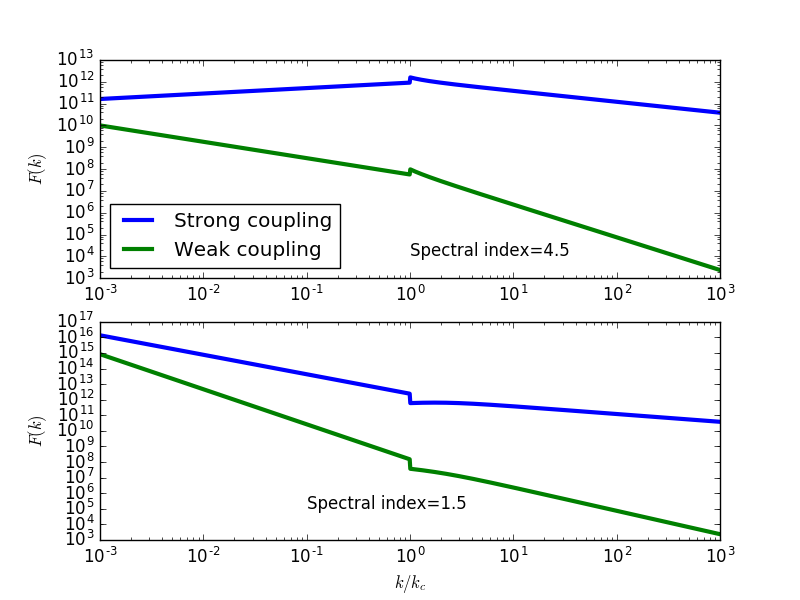
\includegraphics[scale=0.5]{wnm_f(x).png}
	\caption{Exemple de détermination numérique des fonction $F(k)$ dans un WNM. Les fonctions sont tracées suivant le paramètre $k/k_c$ où $k_c$ est relié à $E_c$ l'énergie de coupure de la distribution de l'espèce considérée de rayons cosmiques. Ici on a choisi $E_c = 1~\mathrm{GeV}$. Deux régimes différents sont représentés : l'un dont le spectre de puissance est doux, l'autre avec un spectre dur. Comme $p \propto 1/k$, on remarque que la partie de gauche de chaque graphe possède un intérêt moindre à mesure que le rapport $k/k_c$ diminue et ceci dépendant de la brutalité de la coupure en $p_c \propto 1/k_c$. De manière générale, on remarque que les fonctions $F(k)$ ont une amplitude très élevée et ceci implique (sauf erreur) un gradient de densité de rayons cosmique extrêmement faible. Les constantes choisies sont moyennées.}
\end{figure}





\end{document}